\documentclass{beamer}
%\usetheme{Singapore}
\usetheme{Warsaw}
%\usetheme{Boadilla}
\definecolor{isshblue}{RGB}{115,161,199}
\setbeamercolor{structure}{fg=isshblue!90!black}
%\geometry{paper=a4paper}

%%%%%%%%%%%%%%%%%%%%%%%%%%%%%   TITLE SLIDE   %%%%%%%%%%%%%%%%%%%%%%%

%\titlegraphic{\hspace*{-6.8cm}\vspace*{-1.6cm}
\includegraphics[width=4.2cm]{/Users/richardz/Dropbox/II/projects/nlgis2/graphs/IISG_logo2_eng}}
%	\title{NLGIS-2 Demo}
\logo{%
	\makebox[0.99\paperwidth]{%
    		
\includegraphics[height=1cm,keepaspectratio]{/Users/RichardZ/Dropbox/II/projects/nlgis2/graphs/logo/IISG_logo2_eng}%
		\hfill%
		%
\includegraphics[height=1cm,keepaspectratio]{/Users/RichardZ/Dropbox/II/projects/nlgis2/graphs/logo/nlgis_logo_edit}%
		}%
}	
\subtitle{}
\author[Hoekstra, Rijpma \& Zijdeman, Tykhonov \& de Vries]{Rinke Hoekstra \inst{4} \and%
	Auke Rijpma \inst{3} \and%
	R.L.~Zijdeman \inst{1,2}

\institute[shortinst]{\inst{1} International Institute of Social History \and %
                      \inst{2} University of Stirling} %
                      \inst{3} Utrecht University %
                      \inst{4} Free University

\begin{document}
	\begin{frame}
		\titlepage 
	\end{frame}

%%%%%%%%%%%%%%%%%%%%%%%%%%%%%   OUTLINE   %%%%%%%%%%%%%%%%%%%%%%%
	\begin{frame}
		\frametitle{Outline}
			\tableofcontents[]
		\end{frame}

%%%%%%%%%%%%%%%%%%%%%%%%%%%%%   BACKGROUND   %%%%%%%%%%%%%%%%%%%%%%%
\section{Background}

\begin{frame}
	\frametitle{Twitter}
	\begin{itemize}
		\item \#nlgis 
		\item @rlzijdeman
	\end{itemize}
\end{frame}

\begin{frame}
	\frametitle{Meaning and purpose of GIS}
		\begin{itemize}
        			\item Geographic Information System
			\item Purpose
			\begin{itemize}
				\item{capture, store \& manage data}
				\item{analyze data}
				\item{present data}
			\end{itemize}
		\end{itemize}
\end{frame}


\begin{frame}
	\frametitle{Dutch GIS: Past, Present, Future}
	\begin{itemize}
		\item Kaartgis / NLGIS
  		\item HISGIS.NL (extremely detailed, but not temporal)
		\item NLGIS-2 (detailed and temporal)
	\end{itemize}	 		
		\makebox[0.7\paperwidth]{%
		\hfill%
    		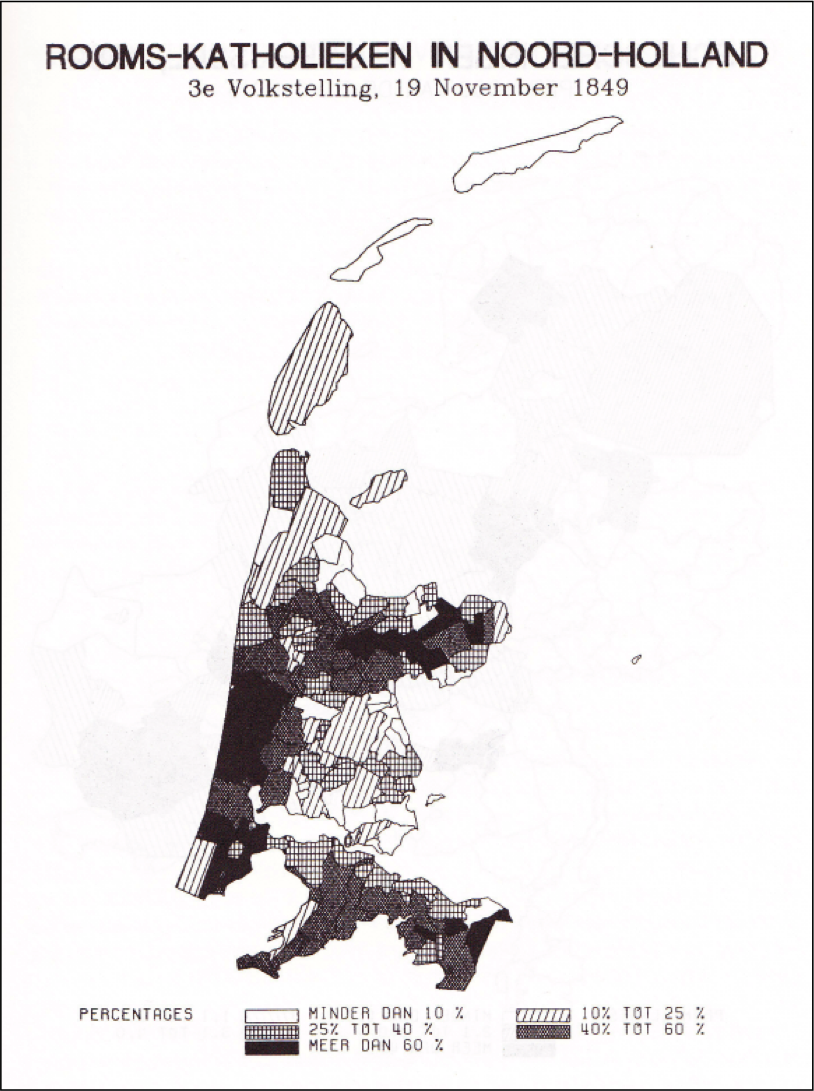
\includegraphics[height=4.5cm,keepaspectratio]{/Users/RichardZ/Dropbox/II/projects/nlgis2/graphs/nlkaart_NH_RK_1849}%
		}%
	
\end{frame}

%%%%%%%%%%%%%%%%%%%%%%%%%%%%%   Goal   %%%%%%%%%%%%%%%%%%%%%%%

\section{Goals}
\begin{frame}
	\frametitle{Goals}
	\begin{itemize}
		\item To disclose the Historical Database of Dutch Municipalities (HDNG)
		\item To plot data from HDNG and other sources on NLGIS' maps 
		\item ... and to do so for a period of five years
	\end{itemize}	
\end{frame}

%%%%%%%%%%%%%%%%%%%%%%%%%%%%%   Approach  %%%%%%%%%%%%%%%%%%%%%
\section{Approach}
\begin{frame}
	\frametitle{Components}
	\begin{itemize}
		\item Maps server (API)
		\item Data server (API) 
		\item Tools to combine maps, data and draw maps
			\begin{itemize}
				\item basic mapping:~website
				\item advanced mapping:~R,  QGIS \& Python
			\end{itemize}
	\end{itemize}
\end{frame}


\begin{frame}
	\frametitle{Sustainability}
	\begin{itemize}
		\item Modular approach:~separating maps and data
		\item Use of main stream open source software
			\begin{itemize}
				\item D3, Leaflet, MongoDB, Python, R
				\item Used by major companies (e.g.~Google, New York Times)
				\item Usable by different types of audiences
			\end{itemize}
	\end{itemize}
\end{frame}


\begin{frame}
	\frametitle{Audience}
		Dual approach:
		\begin{itemize}
			\item No experience with GIS (website)
				\begin{itemize}
					\item Compare regional differences in a phenomenon
					\item Compare changes over time
				\end{itemize}
			\item Advanced users (familiar with QGIS, Python, R)
				\begin{itemize}
					\item Retrieve data from HDNG
					\item Map other datasets
					\item Map outcomes of (advanced) analyses
				\end{itemize}
		\end{itemize}
\end{frame}
%%%%%%%%%%%%%%%%%%%%%%%%%%%%%   Demonstration  %%%%%%%%%%%%%%%%%%%%%

\section{Demonstration}
\begin{frame}
	\frametitle{Website - Demo}
	Features
		\begin{itemize}
			\item HDNG data selection
			\item Information box
			\item Colours
			\item Upload own data
		\end{itemize}
\end{frame}

\begin{frame}
	\frametitle{R - Demo}
	Features
		\begin{itemize}
			\item Functions: nlgget, nlgmap
			\item Main packages: jsonlite, rgdal, leafletR
%			\item Use cases: 
%				\begin{itemize}
%					\item NLGIS meets CEDAR
%					\item NLGIS meets New York Library Map Wrapper
%				\end{itemize}		
		\end{itemize}
\end{frame}




%%%%%%%%%%%%%%%%%%%%%%%%%%%%%   Outlook  %%%%%%%%%%%%%%%%%%%%%
\section{Summary and perspectives}
\begin{frame}
	\frametitle{Summary}
	Features
		\begin{itemize}
			\item easy access to HDNG
			\item easy access to Boonstra maps
			\item easy plotting facility of own and HDNG data
			\item easy access to code through Github
		\end{itemize}
\end{frame}


\begin{frame}
	\frametitle{Summary}	
	Resilience
		\begin{itemize}
			\item 5 years of support by IISH
			\item modular approach
			\item multiple outputs
			\item all data driven, rather than technology driven
		\end{itemize}		
\end{frame}

\begin{frame}
	\frametitle{Perspectives}
	Outlook
		\begin{itemize}
			\item Extend maps beyond 1997
			\item Write codebook for Historical Database Dutch Municipalities (HDNG)
			\item Allow for upload of different kinds of maps (integration with Clariah)
		\end{itemize}
\end{frame}

\begin{frame}
	\frametitle{Connecting the dots}
	The dots:
	\begin{itemize}
		\item Amstedam Code in RDF $\leftarrow$ Gemeentegeschiedenis.nl (Hic Sunt Leones!)
		\item Dutch Historical Census Data $\leftarrow$ CEDAR
		\item Plotting historical data in R $\leftarrow$ NLGIS
		\item Old school maps $\leftarrow$ New York Library
		\item Interactive Plotting $\leftarrow$ Christian Graul's LeafletR
	\end{itemize}
\end{frame}



\end{document}

%%% use \pause if you want to break between visualisation of bullets: i.e.

%\begin{frame}
%	\frametitle{Vindplaats}
%		\begin{itemize}
%			\item Bijv. DANS EASY: https://easy.dans.knaw.nl/ui/home
%				\begin{itemize}
%					\item Overzichtelijk zoeken op kernbegrippen
%					\item Weergave per item en categorie
%					\item Identifiers van datasets
%				\end{itemize}
%			\pause
%			\item Nog te wensen: 
%				\begin{itemize}
%					\item Internationale koppeling van archieven
%					\item Zoeken op variabele-namen
%				\end{itemize}
%			\end{itemize}
%
%			\pause
%			\begin{center}
% 				{\includegraphics[scale=0.5]{/Users/richard/Dropbox/UU/projects/surf/images/variable_selection}}
%   			\end{center}
%\end{frame}
